\chapter{ネットワークアクセス層(その2) 複数の端点を結ぶネットワーク}



ネットワークとは、共有する通信路を介して、相互に直接通信が可能な端点と、その通信路であるとします。では、複数の端点を結ぶネットワークとはどんなものでしょうか。

ここでは、例外はありますが、「誰かに中継してもらわなくても複数の相手と相互に通信できる範囲」であると考えることにします。
本章では、その考えに基づいて、ネットワークアクセス層で、複数の端点を相互に接続するネットワークについて説明をしていきます。


\section{複数の端点を結ぶネットワーク}
複数の端点を結ぶネットワークの特徴は、一対一のネットワークの特徴と全く逆である。自分以外の相手に、区別してもらうための名前なりアドレスなりを全ての端点が持っている。

そして、宛先としてそのアドレスもしくは名前を使い、複数の端点が共有する通信路の上で、特定の相手と通信を行う。

\subsection{ブロードキャストとマルチキャスト}
複数の端点を結ぶネットワークを考えるとき、一対一のネットワークにはない概念が登場する。それは、データの送信先の、その宛先を指定する方法として、ブロードキャストとマルチキャストという概念が現れることである。

ブロードキャストは、同じネットワークの中に接続された端点全てが受信しなければならない通信である。これは、宛先にかかわらず全ての受信者が受信し、処理しなければならない。そのため、一斉放送という意味でブロードキャストという名前が付けられている。

マルチキャストは、同じネットワークの中に、それを受信する必要がある端点が複数ある場合の通信である。受信する側は、宛先のマルチキャストアドレスを参照して、自分が受信しなければならない場合のみ受信し、処理を行う。

最もこれらの概念は、ネットワークアクセス層に固有のものではない。次章以降で説明する、インターネットプロトコル層でも、同様の会年を用いる。だが、ネットワークアクセス層のそれと、インターネットプロトコル層のそれを区別するよう、注意したい。

\section{イーサネット}

では、複数の端点を結ぶネットワークの代表格であり、現在ではLANを構成する規格としてどこででも使用されているイーサネットについて解説しよう。

イーサネットは伝送媒体にケーブルを使用する方式、つまり有線である。だが、イーサネットの技術はALOHAという、無線によるデータ通信技術を基にしている。そのため、無線通信であったことに由来する性質や問題がある。なにより、イーサネットのトラブルはそれを理解していないからこそ「発生させてしまう」ことが多い。

\subsection*{}
\begin{itembox}[l]{いもうとコラム イーサネットの歴史}
まずは、イーサネットの大まかな歴史を追いかけてみましょう。イーサネットの起源までさかのぼれば、その歴史は1960年代後半のハワイ大学にはじまります。

\begin{description}
\item[1960年後半]ハワイ大学で、イーサネットの原型であるALOHA-netの構築が行われました。このALOHA-netは無線ネットワークでした
\item[1972年]XeroxのPARCでロバート・メトカーフがALTO ALOHAネットワークの実験を行いました。これが初のイーサネットの実装です。ALTO ALOHAは、PARCで開発されていたALTOのネットワーク構築に用いられました。通信速度はALTOのクロックに準拠した2.94Mbps\footnote{ALTOのベースクロックが5.88MHzでした}
\item[1973年]メトカーフによって、はじめてEthernetの名称が用いられました同年、特許出願
\item[1976年]メトカーフがNCC(National Computer Conferende)でイーサネットの概念を発表
\item[1977年]イーサネットの特許を米国で取得
\item[1978年]イーサネットリピータの特許を取得。このときまではイーサネットはXeroxの独占でした。
\item[1979年]DEC,Intel,Xeroxの三社がDIX仕様を公開。Xeroxが特許を開放しました。このときの速度は10Mbps
\item[1980年]DIX仕様をベースに、IEEEにEthernet1.0として提出
\item[1985年]IEEE802.3 Carrier Sense Multiple access with Collision Detection(CSMA/CD) Access Method and physical Layer Specification策定。同年、802.3aとして10Base2シンイーサネットと802.3c 10Mbpsリピータの規格も策定されました。
\item[1990年]IEEE802.3i 10BaseT策定
\item[1995年]IEEE802.3u 100BaseT及びAuto Negotioation策定
\item[1999年]IEEE802.3ab 1000BaseT策定
\end{description}

\end{itembox}


\subsection{ALOHA}

イーサネットの歴史的経緯をひもとくと、必ずALOHAという無線ネットワークの名称が出てくる。このALOHAを有線化したのが、最も初期のイーサネットである。では、最初にALOHAがどのようなネットワークであったかの説明を行なおう。

ALOHAとは、1960年代後半から1970年代前半にかけて構築・運用された、ハワイ諸島に分散設置されたハワイ大学の施設と中央のホストコンピュータを結ぶネットワーク、ALOHA-netで使用された方式である。\footnote{ネットワークの直径400Kmであった}当時のハワイは電話線の品質が低く、専用ケーブルを引く費用は莫大であったため、無線によるネットワークが構築された。

ALOHA-netでは、全ての拠点で同一の無線周波数を使用した。そのため、複数の拠点が同時に電波を出したときに発生する混信を回避する制御が必要となることが判明し、それが機能として実装されていった。つまり、同一の伝送媒体を複数の端点が共用するネットワークであったわけだ。

では、そのALOHAの進化の過程についてk、簡単に説明していこう。

\subsection{pure ALOHA}

一番最初に、ALOHA-netの通信方式として実用化されたものを、特にpure ALOHAという。pure ALOHAの通信手順は、以下のような簡単な者である。

\begin{enumerate}
\item 送信者は任意のタイミングでパケットを送出
\item パケットを正常に受信したら、受信者は、受信完了を伝える符号のACKを送出
\item 一定時間内にACKが戻らなければ送信者は再送出
\end{enumerate}
送信タイミングは完全に任意であり、他のホストが送信を行っていても、とりあえず送信を開始してしまう。そのため、混信が多く発生した。そのため、単位時間で有効なデータを送信できるという意味のスループットは 18%程度であった。\footnote{つまり、混信による時間消費、再送などに82%が消費されていたことになる。}

\subsection{改良型ALOHA}

ALOHAの運用によって、単一の無線周波数を複数の拠点からの送受信に使用する、つまり、共有の伝送路を複数の拠点が使用するには、その利用を制御する必要があることが判明した。ALOHAの改良についても簡単に説明しよう。

\subsubsection{Slotted-ALOHA}

ALOHA-netの通信効率を改善するために、時分割したスロットを単位としてデータを送出するSlotted-ALOHAが登場した。これは、同期した時計を使い、送信可能な時間枠をスロットとして管理する。それによって、衝突したスロットのデータを特定し、それだけ再送すればよいようにした方式である。\footnote{時間によって送信できるノードを制限する方式ではない。あくまで、衝突したデータの切片を明らかにするために時計を用いただけである。}Slotted-ALOHAによって、ネットワーク利用率が36\% まで向上した。

\subsubsection{r-ALOHA}

Slotted-ALOHAの改良としてr-ALOHA(reservation-ALOHA予約ALOHA)という方式ができた。これは予約情報を先行して送信し、それを受信した他ノードは送信を行わないという方式である。送信を行う拠点は、予約に成功したのを確認してから送信する。予約の確認とは、予約後一定時間他のホストが電波を出さなかったことを確認することである。その後、送信を行う拠点はパケット送信を開始する。

この方式は、予約を行い、その成功を確認するというオーバヘッドがある。だが、それは確率的に発生する混信で失われる時間よりも小さい。

その後更に、ALOHA-Reservationという予約方式を改良したALOHAも運用されている。だが、本書ではそのような改良が行われたという記述に留めることにする。

\subsection{ALOHAとはどんな通信方式であったのか}

ここで、ALOHAとはどのような通信方式であったか、それを見直してみよう。

\begin{itemize}
\item 伝送媒体を共有する。単一の終発数の電波を使用するので、どこかが送信中は、伝送媒体を専有させる必要がある。
\item 自分が送信したパケットは、自分に返ってこない\footnote{理想環境での話なので、地形や電離層で反射することは考えない。}。つまり伝送路におけるループは存在しない
\item 送信は、全ての拠点で受信可能である。一対一の通信路を確保しない。逆に全ての拠点は伝送路を常時監視する、つまり常時受信待ちを行い、何かパケットが受信できた場合、自分宛化を判別する。自分宛でない場合はその場でパケットを捨てる。
\item 送信する側は、受信する側に事前の連絡は行わない。受信する側が受信することを期待するのみである。
\end{itemize}

これらのアイディアを有線のネットワークに持ち込んだのが、メトカーフであり、次に説明するALTO ALOHAの実装である。

\subsection{ALOHAからALTO ALOHA、そしてイーサネットへ}

現在の、UTP(Unshielded Twist Pair 遮蔽なし撚り対線)とHUBを使用するイーサネットからは、無線通信を祖とした姿をイメージするのは困難である。イーサネットの祖が無線通信であった歴史を見るために、最初のイーサネット実装であるALTO ALOHAまで戻ることにしよう。

1972年、ロバート・メトカーフは、空中に電波を流すかわりに、電気信号の伝送に使用する同軸ケーブルを伝送媒体とした、有線のALOHAネットワークを構築する。当時はまだイーサネットという名前ではなく、パロアルト研究所のコンピュータ、ALTOを結ぶALOHA方式のネットワークということで、ALTO ALOHAという名称が付けられた。

同軸ケーブルとは、電気信号を伝送するケーブルである。身近なところではテレビのアンテナ線に使われているので、目にしたり取り扱ったりすることも多いであろう。構造を簡単に説明すると、中心に信号を伝送する内部胴体があり、その周りにポリエチレンなどの絶縁体がある。その外部にメッシュ状の外部導体、一番外側がビニールなどの保護皮膜となる。外部導体がシールドとなるので、外のノイズが内部導体に乗ったり、内部導体の信号が外に向けて放出されにくい構造となっている。

ALTO ALOHAの伝送媒体は、両端にターミネータをつけた1本の同軸ケーブルであった。ターミネータとは、終端抵抗器と呼ばれることもある電気素子である。ケーブルの端に達した電気信号が反射して、ケーブルの中を戻っていかないように、エネルギーを消費させる役目を持つ。\footnote{無線通信では、試験のためにアンテナと同様の電気抵抗を持つが、電波を発射しないダミーロードと呼ばれる抵抗器を用いることがある。これも、原理と目的はターミネータと同様である。ターミネータがない場合は、開放端から信号が電波として飛んでいったり、反射してケーブルの中を帰ってきたりする。}わかりやすくいうと、信号の発信者から見たときに、理想的な空中のように、送信した信号が自分のところに戻ってくることがない伝送媒体を用意した。

では、各ホストから伝送媒体である同軸ケーブルには、どのように接続するのだろうか。ALTO ALOHAでは、同軸ケーブルの内部導体を伝送媒体として信号を送受信する装置、トランシーバを、同軸ケーブルに直接取り付けた。このトランシーバが、コンピュータと接続され、同軸ケーブルの上を流れる信号を受信し、同軸ケーブルに対して信号を送信した。

ALTO ALOHAがEthernetという名称になるのは、翌1973年のことである。
このALTO ALOHAの構造が、そのままイーサネットの基本原理として40年近く使い続けられていくこととなる。

\begin{figure}[htbp]
	\includegraphics[width=12cm,clip]{draw/altoaloha.eps}
	\caption{ALTO ALOHAの概念図}
	\label{fig:altoaloha}
\end{figure}

\subsection{トランシーバ}

ALTO ALOHAにおけるトランシーバ(Transciever)とは、どのような装置なのであろうか。その答えを先に書いてしまえば、ALTO ALOHAのトランシーバは、同軸ケーブルに対して、信号の送信と受信の両方が可能な装置という意味である。

トランシーバという言葉で、無線通信用の手持ちの無線機を思い浮かべる人も多いであろう。このように、トランシーバという言葉に、なんとなく「無線でお互い話ができる機械」というとらえ方をしている人も多いと思われる。そこで、トランシーバについて簡単に説明をしよう。。

トランシーバ(Transciever)という言葉は、送信機と受信機(Transmitter-Reciever)の合成語である。その意味は、送信機と無線機が一つの箱に入った機械、ということである。

もともと無線機は、送信機と受信機が分かれていた。それだと持ち運びに不便ということで、送信機と受信機を一つの箱に入れるようになる。そうすると、送信機と受信機の両方に存在する、電源系やチューナーなど、一部の電気回路の共用も可能となった。そうして、送信と受信の両方ができる機械として、トランシーバが成立したという経緯がある。だが、送信機能と受信機能は基本的に別回路として構成され、同じ箱に入っているにすぎない。

\subsection*{}
\begin{itembox}[l]{いもうとコラム イーサネットという名前}
Ethernetという名称は、共有伝送媒体を、真空中で電磁波を伝播する仮想の媒体「エーテル」に見立てた名称です。物理メディアが全てのホストにビット列を伝播する様子が、光の伝播媒体であるとされたluminiferous etherと同じであるとして、イーサネットという名前がつけられました。

イーサはエーテルの英語読みです。なお、エーテルの存在は現在では否定されています。電磁波の伝送媒体としてのエーテルの存在を否定したのが、有名なマイケルソン・モーリーの実験です。つまり非実在(ry
\end{itembox}

\section{イーサネットにおける共有伝送媒体の制御}

ALOHAでは、共有する伝送媒体、つまり、同じ周波数の電波をどう管理し、複数の拠点が同時に送信する「衝突」を回避するか、それが改良の歴史であった。では、イーサネットでは、ALOHAの知見と成果をどのように取り入れたのだろうか。

イーサネットでは、共有する伝送媒体である同軸ケーブル、に二つ以上のホストが同時に信号を出さないようにする、「調停」を行う。その調停方法は、CSMA/CD(Carrier Sense Multiple Access/Collision Detect キャリア検知多重アクセス/衝突検出)という名前である。では、CSMA/CDはどのような手順で調停をするのだろうか。。

ここからの説明では、一度に送信される一連の信号を、フレームと呼ぶことにする。イーサネットを流れる一連の信号は、イーサネットフレームと呼ばれる。

\begin{enumerate}
	\item データを送信する前に、伝送媒体上に、最短4マイクロ秒、最長9.6マイクロ秒の信号を送信するだけの時間、信号が流れていないことを確認する。これは、 10Mbpsで、40ビット~96ビットを送出する時間に相当する。
	\item 信号が流れていなければ、伝送媒体に信号を発信する。
	\item 伝送媒体が使用されていないときに信号を送る権利は、全てのホストで等しい。優先順位はないし、特権的に調停を行うノードも存在しない。  \item 信号を送信するホストは、送信中を含む常時、伝送媒体を監視する。他の信号と衝突した場合は、直ちに送信を中止する。その際JAM信号と呼ばれる特別な信号送信して、各ホストに現在受信したフレームを破棄するよう通知する。
	\item JAM信号送出後、ランダムな時間待ったのちに再度送信を試みる
\end{enumerate}

イーサネットでは衝突は必ず発生する。これは異常な状態ではなく、共有の伝送媒体状を有限の速度の電気信号が伝播していくので、タイミングによっては「信号が届いていない」状態と、送信しているホストがいない状態が区別できないためである。

衝突が発生した後ははランダムな待ち時間の後に再送信を試みる。そうすることで、次回以降衝突が発生する確率を下げることができる。

CSMA/CDにおいて、Collision Detectという用語は、ALOHAに由来する問題とその解決方法を正直に説明している。だが、それ故に過去ではイーサネットの性能に疑問の余地を与えていた面もある。\footnote{オライリーの「詳説イーサネット」の筆者であるCharles E. Spurgeonは、その誤解を避けるためには、「調停(arbitation)」という用語を使うべきと記している。}



\subsection{衝突の検出とケーブルの総延長・最小フレームサイズ}

\begin{figure}[htbp]
	\includegraphics[width=12cm,clip]{draw/colision.eps}
	\caption{衝突の検出}
	\label{fig:colision}
\end{figure}


伝送媒体である同軸ケーブル上を伝播していく信号は、有限の速度で、トランシーバの接続されている位置からケーブルの両端に向けて進行していく。上記の通り、信号が届いていない状態と送信しているホストがない状態を区別できない。そのため、あるホストがフレームを送信しているときに、他のホストがそれと衝突するフレームを送信することが起こる。繰り返すが、これは障害ではなく、イーサネットでは確率的に起こりうることである。

では、衝突が発生した際に、その衝突を、その原因となったフレームを送出した複数のホスト\footnote{二つのホストからのフレームが衝突するのではなく、二つ以上のホストからのフレームが衝突する。}が検出(Collision Detect)できる条件を考えてみよう。

まず、同軸ケーブルを伝播する電気信号は、注入された点から、両端に向けて光速以下の一定の速度で進行する。この注入された点とは、トランシーバの取り付け位置になる。電気信号の早さは、内部導体に銅を使う同軸ケーブルで、およそ光速の7割とされる。

電気信号が同軸ケーブルを伝わっていく様子は、波の進行をイメージするとよいだろう。\footnote{ALOHAとイーサネットを比較すると、電気信号か電磁波かという違いだけで、どちらも波である} また、波の合成は単純に足し算である。つまり、二つ以上のフレームが衝突すると、その電気信号は、その二つ以上のフレームの波を合成した、「異常な」波形となる。

イーサネットでは、フレームを送信する側は、フレームの送信開始から送信完了までの間、衝突が発生するかしないかを監視する。送信側が衝突の発生を検知できるのは、別のホストが送出したフレームの先頭が、自分が送信している間に届くことで、自分が送信している信号と同軸ケーブル上の信号が一致しない状態になるからである。

送信開始から送信終了まで衝突が起こらないという状態は、フレームが最も遠いところ\footnote{ここでいう最も遠いところとは、同軸ケーブルの長さで考える。純粋に、伝送路の物理的な距離である。}まで伝播するまで、他のすべてのホストが全く送信しないということである。そして、最悪のケースで衝突が起こった状態というのは、フレームが送信したホストから最も遠いホストのトランシーバに伝播する直前に、送信したホストから最も遠いところにあるホストが送信を始めてしまうことである。この最悪のケースで双方が衝突を検知するには、自分が送信したフレームの先頭が、衝突するフレームを送出した相手に届くまでの時間の、倍の時間が必要である。これは、自分が送出したフレームが相手に届くまでの時間と、その信号が到着する直前という最悪のタイミングで相手が送出した信号が自分に届くまでの時間の合計である。

それだけの時間かかって検知できる「最悪のタイミング」の衝突を検知するにはどうすればよいだろうか。それは、自分が送出した信号が、最も遠い位置にいる相手に届くまでの時間の倍の時間、フレームを送出し続けることである。そうすることで、最悪のタイミングで送出された、衝突するフレームの信号と、自分が送出したフレームの信号が合成されて、異常な信号が発生していることで、衝突を検知できる。これを図示したものが、図\ref{fig:colision}である。

ここまでの話で予想がついたかもしれないが、フレームの最小サイズ、フレーム送出時のビット送信速度、、同軸ケーブルの総延長の三つのパラメータは、相互に影響しあう関係にある。フレーム送出時のビット送信速度は、イーサネットの規格ごとの通信速度となる。また、フレームの最小サイズは、互換性維持のために過去の規格と同一の、固定パラメータである。\footnote{GbE以上の規格では、フレームの最小サイズを古い規格にあわせると、ケーブル長が短くなりすぎる。そのため、ジャンボフレームという巨大なフレームを導入することで、ケーブル長を稼いでいる。}そのため、イーサネットのそれぞれの規格では、通信速度で最大のケーブル長が決まると考えて良いだろう。

\subsection{半二重と全二重}

\begin{figure}[htbp]
	\includegraphics[width=12cm,clip]{draw/duplex.eps}
	\caption{半二重と全二重}
	\label{fig:duplex}
\end{figure}

ここまでに説明したCSMA/CDは、同じ衝突ドメインで、あるホストが送信していると、他のホストは受信しかできない。この状況を単純にするためにホスト2台からなるネットワークで考えてみよう。この場合、片方のホストが送信している間は、もう片方のホストは受信しかできない。同時に送信しようとすると、「衝突」が発生する。

このように、二つのホストが相互に通信できるが、送信はどちらかしかできない通信方法を、半二重(half-duplex)という。つまり、片方が送信しているときは受信、というように、送受信を交代して通信を行うわけだ。

HUBとホストの接続を説明した際、、ホストのTDとHUBのRD、HUBのTDとホストのRDが接続される信号交差が行われている。信号交差を行っているということは、それぞれ信号の伝達をする方向が決まっている、いわば、「上り」と「下り」の経路が別々に存在する。そこで、「経路が別なんだし、送信と受信を同時にやってもいいんじゃね?」というアイディアに繋がった。このような、送信と受信を同時に行う通信方法を、全二重(full-duplex)という。

全二重は、二つのホストが一対一で接続して通信する場合のみ成立する。便宜上、このホストにAとBという名前をつけて説明していこう。AからBに信号を送る経路と、BからAに信号を送る経路が、それぞれ別に存在しなければならない。また、このAとBの間の経路を、第三のホストCと共有することはできないということである。。

では、一対一で、送信と受信の線が別々にあると、イーサネットではどんな利点があるのだろう。それは、CSMA/MDでいうところの「衝突」が発生しなくなる。つまり、CSMA/CDによる制御を行う必要がなくなるということである。

また、全二重方式では、AからBへの送信と、BからAへの送信を同時に行うことができる。実効的に、表記された通信速度の倍で通信することが可能となる。たとえば、100BaseTXというイーサネットの規格では、全二重方式を用いることができる。その場合、AからBへの送信とBからAへの送信で、それぞれ100Mbpsで通信することが可能となる。つまり、単純に計算すれば200Mbpsで半二重通信しているのと同じになる。

繰り返すが、イーサネットで全二重方式を実現するには二つのホストの間で一対一の通信を行わなければならない。つまり、衝突ドメインが存在してはならない。つまり、全二重はスイッチングHUBのみでサポートされる。また、伝送媒体で、送受信の往復には別の経路が存在しなければならない。

逆に、全二重方式のみで構成されたネットワークは衝突ドメインが存在しないと言うこともできる。これは、接続された機器が全て一対一通信を行い、送受信の往復に別の伝送経路を使用するということである。つまり、ALOHAに由来するイーサネットの基本、複数の機器が共有して使用する伝送媒体というものが存在しなくなることである。



\subsection*{}
\begin{itembox}[l]{いもうとコラム 全二重と半二重のマッチング}
現在では、イーサネットのネットワーク機器を相互に接続した場合は、全二重、半二重のマッチングは、多くの場合自動で行われます。そのため、全二重、半二重を明示的に指定しなければならない場面はあまりありません。また、多くの場合は、機器が自動で全二重の通信を選択します。

ですが、業務用のネットワーク機器など、手動で明示的に全二重と半二重どちらを使うか設定することができる機器も、多く存在します。

では、自動で行われるマッチングが失敗したり、手動での設定を間違えて、ホストの一方が全二重、もう一方が半二重で通信しようとした場合は、何が起こるのでしょうか。

全二重と半二重のミスマッチングが発生している場合、はっきり分かる現象として、通信が遅くなります。\footnote{接続したネットワーク機器間の通信が異常なレベルで遅い場合は、全二重、半二重のネゴシエーションの失敗や設定ミスを疑ったほうがいいでしょう。}これは、片方がCSMA/CDに従って通信を行っているのに対し、もう片方がCSMA/CD手順関係なしに送信を行うためです。

そのため、半二重側から見たとき、衝突の発生頻度が高くなります。その結果、通信速度が遅くなるというわけなのです。

一方、全二重側から見ると、通信の相手は高い確率で通信の中断を求めるJAM信号を送信してくるように見えます。そのため、確率的に、単位時間内で成功する送信が減り、結果、通信速度が遅くなるというしくみです。\footnote{実際には、トランスポート層の応答待ちなどで、イーサネットで通信が遅くなることがトリガーとなって、雪達磨式にアプリケーション層の通信の遅延の原因となっていきます。}
\end{itembox}





\section{イーサネットでホストを区別する}

\begin{figure}[htbp]
	\includegraphics[width=12cm,clip]{draw/macaddr.eps}
	\caption{MACアドレスの構造}
	\label{fig:macaddress}
\end{figure}

本章の冒頭で、複数の端点が通信経路を共有するネットワークでは、端点を区別するための名前もしくはアドレスが必要になる、という話をした。では、イーサネットでは、どのようにお互いを区別しているのだろうか。

イーサネットは、一つのホストが送信した信号を、全ホストで受信し、自分宛でないフレームは破棄するというALOHA以来の方法で、特定の宛先にフレームを届けている。そのため、イーサネットでは、共有の伝送媒体に接続されたホストを区別する方法が必要になる。

その区別を行うのに、MAC(Media Access Control メディアアクセス制御)アドレスという48bit(6octet)長のアドレスを使用する。このMACアドレスは、イーサネットのフレームを送受信する全てのインタフェイスに、世界唯一のユニークなものとして割り当てられる。つまり、ネットワーク内で重複することがない。そのため、イーサネットのプロトコルには、ホストのインタフェイスにMACアドレスを割り当てたり、同じネットワーク上のMACアドレスを管理したりする仕組みがない。



MACアドレスの構造は、図\ref{fig:macaddress}のように、48ビット長のアドレスである。
MACアドレスはネットワークインタフェイス毎にユニークであり、上位24ビットがベンダに割り当てられたOUI(Organizationally Unique Identifier 管理組織識別番号)となる。このOUIは、ベンダコードと通称されることが多い。また、下位24ビットが、ベンダがネットワークインタフェイスに割り当てるアドレスとなる。

MACアドレスには、同じ同軸ケーブルに接続されているの全てのホスト宛を意味するブロードキャストアドレスと、その中で特定のグループをつくり、グループに属するホスト全てのみを宛先とするマルチキャストアドレスとがある。これは、上位層のブロードキャストアドレス、マルチキャストアドレスとは別のものである。

\subsection{イーサネットの通信手順}

イーサネットでの通信手順を、MACプロトコルという。このMACプロトコルが、前述したCSMA/CDとMACアドレスを使用して、どのような手順で行われるかを説明しよう。
\begin{enumerate}
\item ホストは、通常は共有通信チャネルを監視する。共有通信チャネルとは、同じネットワークを構成するための伝送媒体である。
\item あるホストが送信するときは、前述のCSMA/CDの手順で行う。
\item 共有通信チャネルに送り出されたイーサネットフレームがあれば、とりあえず受信する。その後、宛先を自分のMACアドレスと比較、同じであればヘッダとフッタを抜いたデータ部分を上のレイヤに渡す。自分のMACアドレスと一致しなければ、そのフレームは無視する。
\end{enumerate}

MACプロトコルの動作は、これだけしかない。イーサネットでは、同一の伝送媒体にフレームを送信し、同一の伝送媒体に接続されている全てのホストで受信する。その後、自分宛でないデータは破棄するという手順である。

イーサネットは、送信が全てのホストで受信可能であることから、ブロードキャスト型の通信と言われることがある。

また、イーサネットでは、エンドツーエンドの通信路を確保したり、受信の確認を送出したりはしない。イーサネットでは、相手が受信したことを期待するだけである。確実な通信を行う必要があれば、上位層のレイヤが、イーサネットを通信手段に使って行うであろう。そして、TCP/IPにおいて確実な通信を行うために何かをするのは、トランスポート層のTCPだけである。イーサネットなど、ネットワークアクセス層の仕事ではない。


\subsection{MACアドレスのブロードキャストアドレス}

MACアドレスには、ブロードキャストアドレスと呼ばれる特別なアドレスがある。ブロードキャストアドレスは、そのネットワークに接続された、全てのインタフェイスを宛先とする。\footnote{インターネットプロトコル層にもブロードキャストアドレスが存在する。それは、ここで説明するMACアドレスのブロードキャストアドレスとは全く別のものである。}MACプロトコルの手順で、全てのホストは、送出されたフレームをいちど受信する。そのフレームの宛先がブロードキャストアドレスであれば、そのフレームは自分宛として処理する。

つまり、ブロードキャストアドレスは、同じネットワークに接続された全てのインタフェイスが受信する宛先アドレスである。ブロードキャストアドレスは、MACアドレスの全てのビットを1にしたものであり、十六進表記するとFF:FF:FF:FF:FF:FFとなる。

ブロードキャストアドレスは、宛先としてのみ指定可能である。送信元MACアドレスとして使用することはできない。

\subsection{MACアドレスのマルチキャストアドレス}
MACアドレスには、マルチキャストアドレスとよばれるアドレスもある。マルチキャストアドレスは、同じネットワークの中で、受信する必要のあるネットワークインタフェイスのみが受信するアドレスとである。。

マルチキャストアドレスは、先頭16bitが、00110011-00110011、つまり16進で33-33となる。

ブロードキャストアドレスと同様に、送出されたフレームは、MACプロトコルに従って、全てのホストに到達する。そして、その宛先アドレスが、自分に似設定されたマルチキャストアドレスであれば、そのフレームを受信する。それが自分に設定されたマルチキャストアドレスでないばあいは、破棄する。

マルチキャストアドレスも、ブロードキャストアドレス同様、送信元MACアドレスにすることはできない。

\subsection{ブロードキャストアドレス、マルチキャストアドレスの区別}
ブロードキャストアドレス、もしくはマルチキャストアドレスを宛先としたフレームは、とりあえず全てのホストのいたフェイスに到達する必要がある。つまり、同じネットワークの中にある中継機器は、それを見分けて中継しなければならない。

ブロードキャストアドレス、マルチキャストアドレスとも、MACアドレスの先頭バイトの最終ビットが1である。ネット枠アクセス層に対応した機器は、それを判別して、全てのインタフェイスに中継をする。

\section{イーサネットの接続と衝突ドメイン}

\begin{figure}[htbp]
	\includegraphics[width=12cm,clip]{draw/collisiondomain.eps}
	\caption{衝突ドメイン}
	\label{fig:collisiondomain}
\end{figure}

ここまで、イーサネットは同軸ケーブルを使用していた、という説明を行っていた。つまり、同じ一本の同軸ケーブルに繋がっている全てのホストが、一つのネットワークを構成しているということである。これは、一本の同軸ケーブルが、「どのネットワークか」という、ネットワークを区別する単位であると言うこともできるであろう。

では、ネットワークを区別する単位である同軸ケーブルが複数あった場合はどうなるだろうか。そして、その複数のネットワークを接続していくことを考えたら、何が起こるであろうか。

同軸ケーブルが複数ある、つまり、ネットワークが複数ある場合に、ネットワークアクセス層のレベルで接続して、一つのネットワークにする方法について説明する。この複数のネットワークの接続を考えるときに出てくるのが、衝突ドメイン(Collision Domain)という概念である。この衝突ドメインは、どのように定義されるのだろうか。

衝突ドメインとは、同じ共有通信チャネルに接続されたホスト全てである。また、その中の一台が送信している間、同じ衝突ドメインになるホスト全てが、CSMA/CDによる調停に従って送信できなくなる。つまり、同じ衝突ドメインに属する複数のホストが同時に送信すると、衝突が発生する

イーサネットにおいて、同じ同軸ケーブルに接続されている、同一のネットワークのホストは、同じ衝突ドメインに属していると言うこともできる。

\subsection{複数の衝突ドメインを接続する}




では、次に、複数の衝突ドメイン、つまり、同軸ケーブルからなるネットワークを相互接続することを考えてみよう。

二つのネットワークを接続する機器は、その機能の違いから二種類存在する。その機器はそれぞれ、リピータ、ブリッジと呼ばれている。リピータとブリッジは、どちらも、二つのネットワークに接続して、接続したネットワークの間で、フレームを中継する機器である。

では、二つのネットワークの間でフレームを中継する、という機能では同じなのに、なぜリピータとブリッジの二種類の機器があるのだろうか。実は、リピータは増幅器として電気的にフレームの信号を中継する機器であり、ブリッジは二つのネットワークに同時に接続してフレームを転送するコンピュータである。このように、フレームを中継するという機能は同じでも、中身が全く異なる機器なのだ。

では、リピータとブリッジについて、もう少し説明をしていくことにしよう。

\subsection{リピータ}

二つのネットワークを、単純に接続して、ひとつの同じネットワーク「するための機器を、リピータ(中継器)という。

接続したネットワーク片方のネットワークでフレームの送信があり、そのフレームがリピータに届いたら、リピータによって、そのままもう片方のネットワークにも伝送される。だが、受信した電気信号ものをそのまま流すのではなく、イーサネットフレームとして再度送り出す。単純に内部でケーブルを接続しているだけではない。

リピータで接続された二つのネットワークは、同じ衝突ドメインとなる。また、ケーブルの総延長という観点で見ると、リピータによる接続は、同軸ケーブルを継ぎ足すのと等価である。

\subsection{ブリッジ}

ブリッジは、二つのネットワーク、つまり、衝突ドメインに同時に接続されるコンピュータである。ブリッジは、中継するフレームの送信元MACアドレスを参照して、それぞれの衝突ドメインにどのMACアドレスをもつインタフェイスが接続されているかを学習する。

ブリッジは、学習したMACアドレスの一覧を持つ。このMACアドレスの一覧は、宛先となる機器が二つあるどちらのネットワークに接続されているかを判断するのに用いられる。フレームの宛先が送信したホストと同じネットワークであれば、ブリッジはフレームをもう一方のネットワークに転送しない。宛先が、送信したホストと違う方のネットワークにあることがわかっている場合、もしくは、そのMACアドレスがまだ一覧表になくて、宛先がどちらのネットワークにあるかわかっていない場合は、ブリッジはフレームをもう一方のネットワークへ転送する。

学習が進んで、それぞれのネットワークに接続されたインタフェイスのMACアドレスをすべて学習したら、違うネットワークにあると分かっているフレーム、もしくはすべてのインタフェイスに届けるフレーム以外は、ブリッジで中継されることがなくなる。

そのため、ブリッジに接続された二本の同軸ケーブルそれぞれの中で完結する通信であれば、ブリッジによって同じネットワークになったにもかかわらず、衝突せずに同時に通信することができる。

つまり、ブリッジで接続されたそれぞれの部分は、同じネットワークであるが、同じ衝突ドメインではない、独立した二つの衝突ドメインとなる。

\begin{figure}[htbp]
	\includegraphics[width=12cm,clip]{draw/repeaterbridge.eps}
	\caption{リピータとブリッジ}
	\label{fig:repeaterbridge}
\end{figure}

\subsection{ネットワークを接続したときの総延長}

ネットワークをリピータで接続して同一の衝突ドメインとした場合、最も離れているホスト同士の距離を、ケーブルの総延長という。

繰り返すが、イーサネットは、CSMA/CDで同一の衝突ドメインで発生する衝突を検知するために、通信速度によってケーブルの総延長が規定される。では、リピータやブリッジで二つのネットワークを接続した場合、そのケーブルの総延長はどのように考えればよいだろうか。

リピータの場合は、接続したケーブルは、論理的に一本のケーブルと見なすことができる。つまり、接続した全てのケーブルの長さを合計して、そのイーサネットの規格で定められたケーブル長より短くしなければならない。

ブリッジの場合は、少し複雑である。接続されるネットワークは、電気的にはそれぞれ独立している。だが、ブリッジは、有限の速度で動作するコンピュータである、フレームからMACアドレスを読み取り、必要であれば適切なネットワークに転送する処理に、ゼロでない時間が必要である。つまり、ブリッジを介した通信に時間が必要であり、それは、ケーブルの総延長が伸びたことと等価である。

ブリッジ接続の場合は、ケーブルの総延長と、ブリッジを何段まで繋ぐかを同時に考慮する必要がある。

\subsection{ブロードキャストフレームの中継}
先ほど、ブロードキャストアドレスは、同じネットワークのホスト全てを宛先としたMACアドレスであると説明した。つまり、ブロードキャストアドレス宛のフレームは、同じネットワークに接続された全てのインタフェイスに届く必要がある。

リピータは、二つの衝突ドメインを連結している。そのため、ブロードキャストアドレス宛を含む全てのフレームは、リピータで接続された、ネットワーク全てに伝播する。

ブリッジは、二つの衝突ドメインを独立した衝突ドメインとしたまま、同じネットワークとして接続する。だが、これまで書いたように、ブロードキャストアドレス当てということは、同じネットワークの全てのホストにフレームが届く必要がある。
そのため、ブリッジは、ブロードキャストアドレス宛のフレームは、全ての衝突ドメインに対して送出する。そうすることで、同じネットワークのインタフェイス全てに、ブロードキャストアドレス宛のフレームが届く。

\subsection{マルチキャストフレームの中継}
マルチキャストフレームが発信された場合、ブリッジはどのような動作をするであろうか。

先に説明したとおり、マルチキャストアドレスは送信元のMACアドレスとすることはできない。そのため、ブリッジがマルチキャストアドレスを受信するホストがどこに存在するかを受信することはない。そのため、ブリッジはマルチキャストアドレス宛のフレームを全ての衝突ドメインに対して送出する。

そのフレームを受信するかどうかは、受信するインタフェイスがマルチキャストアドレスのグループに所属するかどうかで決定される。


\section{現在のイーサネット}

ここまでイーサネットの説明を行ったが、一度もHUBを使用した現在のイーサネットの説明をしてこなかった。それは、イーサネットの動作を理解するには、ALOHA方式や同軸ケーブルを使用していた頃の昔話から入らないと納得できない点が多いためである。

では、現在、イーサネットによるネットワークを構築するのに使用されるHUBとは、ここまで説明してきた何なのだろうか。

HUBとは、集めるもの、中心、というように、「何かを集中させる部分」という意味がある。その名の通り、HUBには、複数のLANケーブルが接続される。HUBにもうけられた、LANケーブルを接続するための口を、ポートと呼ぶ。HUBのポートの数は、そのHUBに接続することができるLANケーブルの数でもある。\footnote{古いHUBでは、他のHUBに接続する専用のポートと、ホストに接続するポートの一つが排他利用となっている場合がある。そのため、必ずポートの数だけホストを接続できるわけではない。}ここから先は、、現在LANに使用されるケーブル、UTPをHUBに接続するという、現代のイーサネットを説明していきたい。

HUBという名前で呼ばれる機器は、リピータHUBとスイッチングHUB(SW-HUB)に分けられる。このそれぞれについて説明をしていくことにしよう。
\subsection{リピータHUB}

リピータHUBの内部をここまでに沿って説明すれば、共有の伝送路である同軸ケーブルと、そのケーブルに取り付けていた複数のトランシーバを一つの箱に置き換えたものと考えればいいだろう。LAN ケーブルを接続するポートのどれかから共有の伝送路に向けて送信されたフレームは、全てのポートに送信される。

そのため、リピータによって構成されたHUBというおkとで、リピータHUBという名称で呼ばれる。つまり、リピータHUBによって構成されるネットワークは、同じ衝突ドメインとなる。

\subsection{スイッチングHUB}

スイッチングHUBは、ブリッジが発展したものである。スイッチングHUBのポートは、すべて独立した衝突メインである。つまり、スイッチングHUBには、ポートの数だけ衝突ドメインがある。

そして、そのポートの数だけある衝突ドメインを全て、相互にブリッジで接続している。古い解説では、クロスバー式の電話交換機のような模式図で描かれることもあった。

では、個々の衝突ドメイン間の接続はのように行っているのだろうか。スイッチングHUBは、ブリッジの集合体と言うこともできる。つまり、コンピュータである。そのメモリ上のテーブルに、ポートごとに接続されている機器のインタフェイスのMACアドレス一覧表を、ブリッジとしての学習で獲得する。そして、あるポートへ送信されたフレームは、この一覧表を参照して、受信するインタフェイスが接続されたポートにのみ、そのフレームを送出する。

ただし、スイッチングHUBも、全てのポートにフレームを送信するブロードキャストを行う場合がある。学習していないMACアドレス宛のフレームを送信する場合と、ブロードキャスト、マルチキャストのMACアドレスを宛先とするフレームは、全てのポートに送信される。

\subsection{LANケーブル}

ここまでで、LANケーブルとUTPという名称を同じ本野として使用してきた。そのUTPとは何であろうか。

UTPとは、Unsielded Twisted Pair(遮蔽なし撚り対線)の略称である。

撚り対線とは外部にノイズを出しにくく、また、ノイズの影響を受けにくい。では、撚り対線がノイズの影響を受けにくい理由について、簡単に説明しよう。

一本のケーブルに電流を流すと、その周囲に、右ねじの法則に従った回転磁束が発生する。その回転磁束が電磁誘導をおこし、エネルギーの一部が電磁波として放出される。逆に、電磁波にさらされているケーブルは、電磁波による回転磁束によって、電磁誘導による誘導電流を生ずる。つまり、ケーブルはそれだけでアンテナになる)。これが、ノイズを出すということであり、ノイズを受けるということである。

撚り対線は、流す電流の向きが逆になるケーブル2本を撚りあわせた構造になっている。電流の向きが逆であるケーブルが撚られているので、撚り合わせ毎に、発生する磁束は、打ち消しあう方向で隣り合う。それによって、撚り対線のそれぞれのケーブルから発生している磁束は互いにうち消しあう。

次に、撚り対線が電磁波にさらされている場合、つまり、撚り対線を横切る磁束がある場合を考えよう。この磁束でより対線には誘導電流が生じる。だが、「撚ってある」形状のため、その誘導電流は一本のケーブルの中で、常にうち消しあう方向に生ずる。

それによって、撚り対線はノイズを出しにくく、ノイズを受けにくい。

\subsection{UTPのカテゴリ}

UTPは、2芯で一対と数える撚り対線を、複数パッケージして1本のケーブルにしたものである。UTPの規格はカテゴリの後に数字をつけてあらわす。表記としては、カテゴリをCat.と省略して書くことが多い。

このカテゴリは、単位長の1フィート(約30cm)あたり、何回撚りあわせてあるかで決められる。たとえば、カテゴリ3では1フィートあたり2回撚り合わせる。カテゴリ5では、ケーブルのメーカによっては19から25回撚り合わせている製品もある。

カテゴリ6の製品では、4対の依り対線を内部で分離するイソレータを入れることになっている。余談ながら、Cat5で芯にイソレーターっぽいなにかとして光ファイバが入っているオーディオ用の製品が存在するが、その効果はオカルトの領分である。

また、カテゴリ毎に何対の接続が必要かという規定はあるが、撚り対線を何対使用しているかは、カテゴリの数字が多いからという理由で多くなるわけではない。たとえば、 ISDNの接続に使用されるUTP カテゴリ2は8芯4対のツイストペアをコネクタに接続しなければならない。だが、10BaseTに使用するカテゴリ3は、4芯2対の接続となる。また、カテゴリ5を使用する 

また、100BaseTXは、その通信には4芯2対しか使用しない。だが、カテゴリ5の規格では8芯4線の接続をしなければならない。そのため、イーサーネットで使用するLANケーブルは、ネットワークの規格を理解した上で、その規格に対応したカテゴリのケーブルを選択する必要がある。



\subsection{UTPとSTP}

\begin{figure}[htbp]
	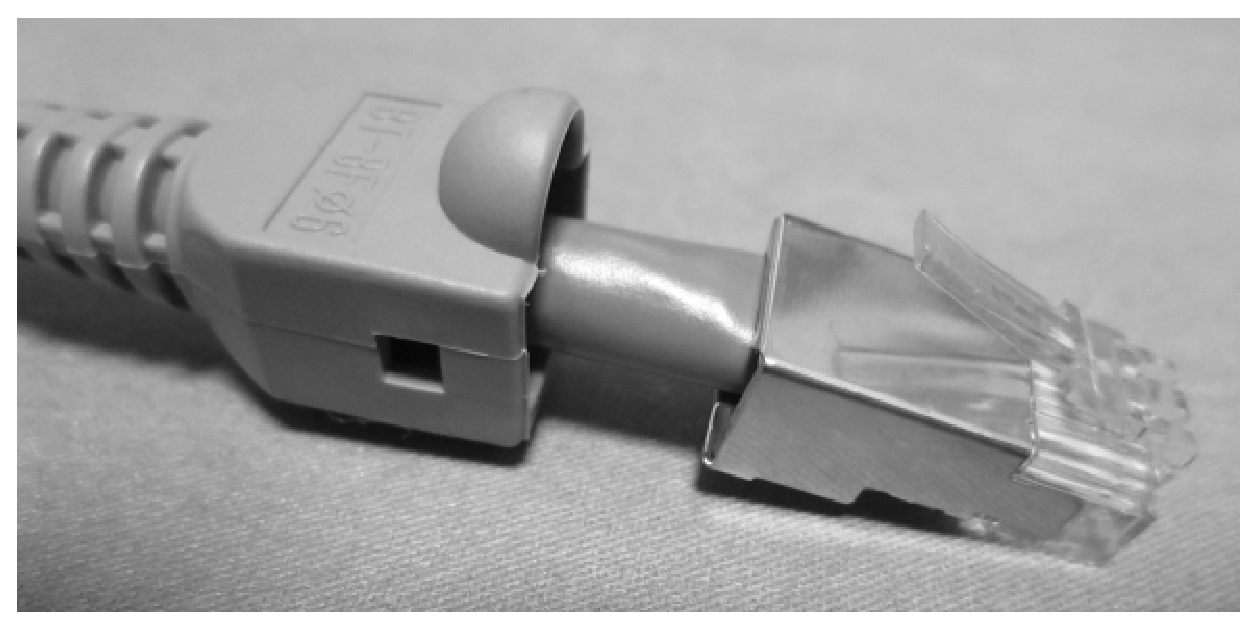
\includegraphics[width=12cm,clip]{draw/stp.eps}
	\caption{STPケーブル}
	\label{fig:stp}
\end{figure}

さて、UTPに関するここまでの説明で、一つ疑問に思わなかっただろうか。撚り対線ならTP(Twisted Pair)でいいのではないか。なぜわざわざUTPと、Unshieldedとつけるのか。

それは、UTPに対してSTP(Shielded TP 遮蔽あり撚り対線)というケーブルが存在するためである。STPは、撚り対線ごとに、同軸ケーブルの外部導体のようなシールドをつけ、よりノイズを受けにくい構造にしたケーブルである。図\ref{fig:stp}でわかるように、コネクタ部分に金属シールドが着いていることがSTPの外見的特徴である。

STPは、特にノイズの多い工場などで使用される。だが、シールドを接地(アース)する必要があるため、ネットワーク機器もSTP対応のものが必要となる。

ヨーロッパで普及している規格であるが、日本では、STP が必要な場面では光ファイバが使用されることが多い。そのため、日本ではSTP対応のケーブルや機器は、あまり見かけることはない。

\subsection{LANケーブルのピンアサイン}

LANケーブルで使用されるRJ-45というコネクタは、8本のピンがある。このピンを2本ずつ接続することで、一対の信号線ができるようになっている。では、実際にLANケーブルの線とコネクタの配線はどのようになっているのだろうか。

\begin{figure}[htbp]
	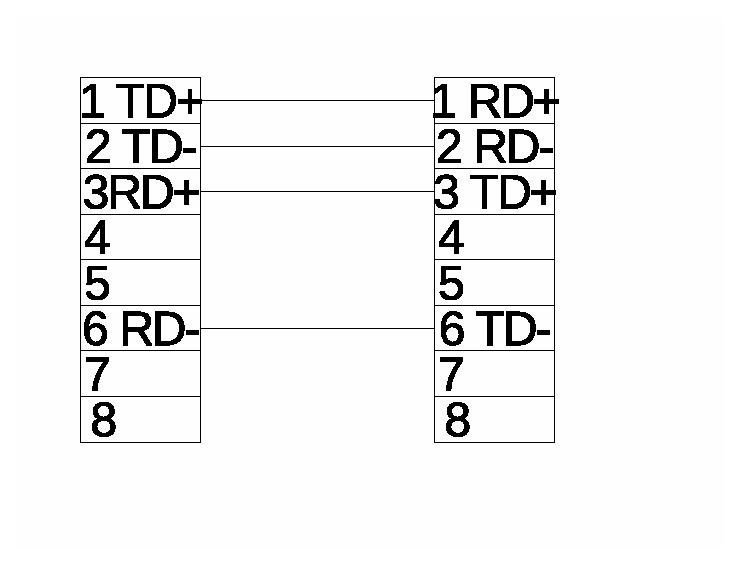
\includegraphics[width=10cm,clip]{draw/cat5pin.eps}
	\caption{10BaseT、100BaseTXのピンアサイン}
	\label{fig:pinassign}
\end{figure}

10BaseT出用いられるCat.3のケーブル、100BaseTXで用いられるCat.5のケーブルでは、各ピンは表\ref{pinassign}のように用いられる。使用されていないピンの間は、配線を省略してある場合がある。図で、TDは送信データ、RDは受信データのためのピンであることを表す。

ツイストペアは、1バント2番、3番と4番、というように、番号が続いているピンにわりあてていく。
Cat.3とCat.5のLANケーブルは、通常、両端のコネクタのピンの、同じ番号同士を結線する。そのため、コネクタに対してこのような結線を行ったケーブルを、ストレートケーブルと呼ぶ。

だが、LANケーブルを使用してネットワークを構成するには、送信側コネクタのTD(送信データ)端子から送信される信号を、受信側ではRD(受信データ)端子で受け取る必要がある。これを、両端の送信と受信の端子を互い違いに接続することから、信号交差と呼ぶ。

だが、HUBとホストの接続ではストレートケーブルを使う。これはなぜであろうか。それは、HUB側のコネクタで、1番と2番ピンに来た信号を受信し、3番と4番から送信する、「信号交差」を行っているからである。つまり、ネットワーク接続するホストの側と、HUBの側では、TDとRDの配置がそっくり入れ替えられている。

では、ホストとホストを直結したり、HUBとHUBを直結したりするというように、ピン配置が同じ機器を接続することはできるのだろうか。そのときは、両端のコネクタの TDのピンとRDのピンを結ぶように結線した、信号交差用のLANケーブルを使用する。
信号交差を行うよう配線したケーブルが、図\ref{fig:cross}のクロスケーブルである。

\begin{figure}[htbp]
	\includegraphics[width=10cm,clip]{draw/cat5cross.eps}
	\caption{クロスケーブル}
	\label{fig:cross}
\end{figure}


最近のHUBのほとんどは、全てのポートで信号交差が必要かどうかを自動判別する機能がある。そのため、ストレートケーブルかクロスケーブルか、つなぐものはホストかHUBかを気にせず使える場合が多い。だが、務用のネットワーク機器には、信号交差が必要か、自動判別を行わないものがある。そのような機器は、ディップスイッチや設定ファイルによって、特定のポートの信号交差を設定する。

\subsection{Cat5eとCat6のピンアサイン}
Cat5eとCat6は、4対8線のケーブルを全て使用する。そのため、図\ref{fig:cat5e}のように、全てのピンを同じ番号のピン同士を配線する。

\begin{figure}[htbp]
	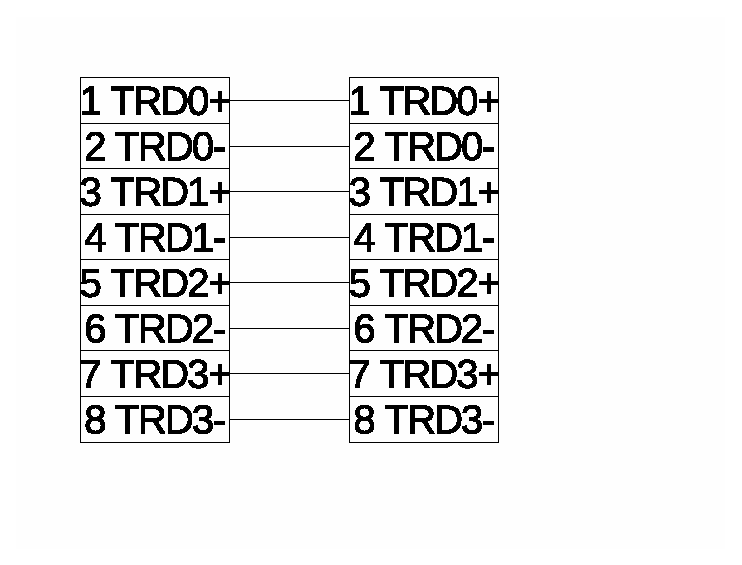
\includegraphics[width=10cm,clip]{draw/cat5e.eps}
	\caption{Cat.5e、Cat.6ケーブル}
	\label{fig:cat5e}
\end{figure}

Cat.5eとCat.6の違いは、イソレータというパーツの有無である。Cat.6は、4対のツイストペアを隔離するイソレータが入っている。

\subsection{カスケード接続}

HUB同士をLANケーブルで接続することを、カスケード接続という。カスケードとは「滝」であり、何段にもなっている滝のようにHUBが接続されている状況を表したものである。では、リピータHUBとスイッチングHUBのそれぞれについて、カスケード接続の説明を行うとどうなるかを説明しよう。

\subsubsection{リピータHUB同士のカスケード接続}

リピータHUB同士をLANケーブルで接続すると、その二つのHUBで構成されるネットワークは、同じ衝突ドメインとなる。リピータHUB同士のカスケード接続は、動作が保証されるのは、信号の速度10Mbpsの10BaseTで4段、100Mbpsの100BaseTXで2段までとされる。

HUBの段数が増えることが、衝突ドメインを構成するネットワークの総延長が延びることと等価であるためである。そのため、カスケード接続の段数は、論理的なケーブルの総延長をを規格内に納めるといういみで制限をされる。

\subsubsection{スイッチングHUB同士のカスケード接続}

次に、スイッチングHUB同士の接続について説明する。これは、同軸ケーブルのときのブリッジが発展したものと考えればよい。つまり、接続されたスイッチングHUBのそれぞれは、同じネットワークであるが、異なる衝突ドメインである。では、ふたつのスイッチングHUBを接続すると、通信はどのように行われるのであろうか。

ここでは、二つのスイッチングHUBのそれぞれを、AとB、と仮称し、そのAとBをカスケード接続する場合で考えていこう。

まず、Aに接続されたインタフェイスの一つからイーサネットフレームが送信されたとする。その宛先が、Aに接続されているインタフェイスのMACアドレスであれば、そのフレームはAの適切なポートに送信される。\footnote{自分自身への送信は、ローカルループバックインタフェイスでバッファリングされ、信号として送出されずに自分からの通信として処理される。}

では、Bに接続されているインタフェイスのMACアドレスを、Aはどのように学習するのだろうか。

BからAに送信されてくるフレームは、全て「Bに接続されている」ポートからくる。そのため、単に、そのポートに接続されている機器のMACアドレスを複数覚えればよい。Bに接続されているホスト宛のイーサネットフレームであれば、Bに接続されているポートに送信する。Bは、MACアドレスとポートの対比表をひいて、フレームを送信するポートを決定する。

Aで全てのポートに送出する必要があると判断されたフレームは、Bの繋がっているポートにも送信される。\footnote{ブロードキャストアドレス宛だけでなく、マルチキャストや未学習の宛先へのフレームの場合もある。}それを受け取ったBは、「Bの中で全てのポートに送出する必要があるか」を判断して、必要であれば全ポートに送出する。

スイッチングHUB同士のカスケード接続は、同じネットワークではあるが、同じ衝突ドメインにならない。だが、スイッチングHUBのカスケード接続は7段が限度とされる。それはなぜだろうか。

スイッチングHUBは、フレームの宛先を読み取り、どのポートに送出するべきかを判断してから適切なポートに送出する。フレームを受信し始めてからどの時点で送出するかでいくつか方式があるが、フレームを受信し始めてから送出するまでの間に、必ず時間差が生じる。この時間差はLANケーブルの総延長が延びていることと同じ意味を持つ。

この遅延は、カスケードするスイッチングHUBの数だけ蓄積される。そのため、衝突を検出できるカスケードの段数は、7段が限界とされている。l

\subsection{スイッチングHUBのJAM信号送出}

先ほど説明したとおり、スイッチングハブは、ポートに到着したフレームをある適度読み込み、宛先のMACアドレスを解釈して、適切なポートに送信する。だが、このメモリの容量は有限である。もし、スイッチングHUBがストア可能なメモリを使いきったら、いったん全ての受信動作を止め、メモリ上のデータを送出する。

また、MACアドレスの学習の結果や、全ポートへの送出で送信したいポートが分かっている状態で、そのポートが別のフレームを送信しようとしている場合もある。

このような場合は、何らかの方法で、その通信に関係するインタフェイスからの通信を止める必要がある。そのための方法として、スイッチングHUBは、擬似的に衝突を発生させる。スイッチングHUBは、CSMA/CDで、衝突による送信の中断を知らせるJAM信号を送出するスイッチングHUBからのJAM信号を受信したインタフェイスは、CSMA/CDに従って、ランダムな時間フレームを送信せずに待つ。

\section{イーサネットとネットワークのループ}

イーサネットは、無線ネットワークのALOHAに由来する。そのため、伝送媒体に送出したフレームが送信者に戻ってくることはない。つまり、伝送媒体にループがあってはならないことはここまでで説明していた。だが、イーサネットでループを作ると、どのような現象が発生するのだろうか。それについて説明を行おう。


\subsection{リピータによるループ}


\begin{figure}[htbp]
	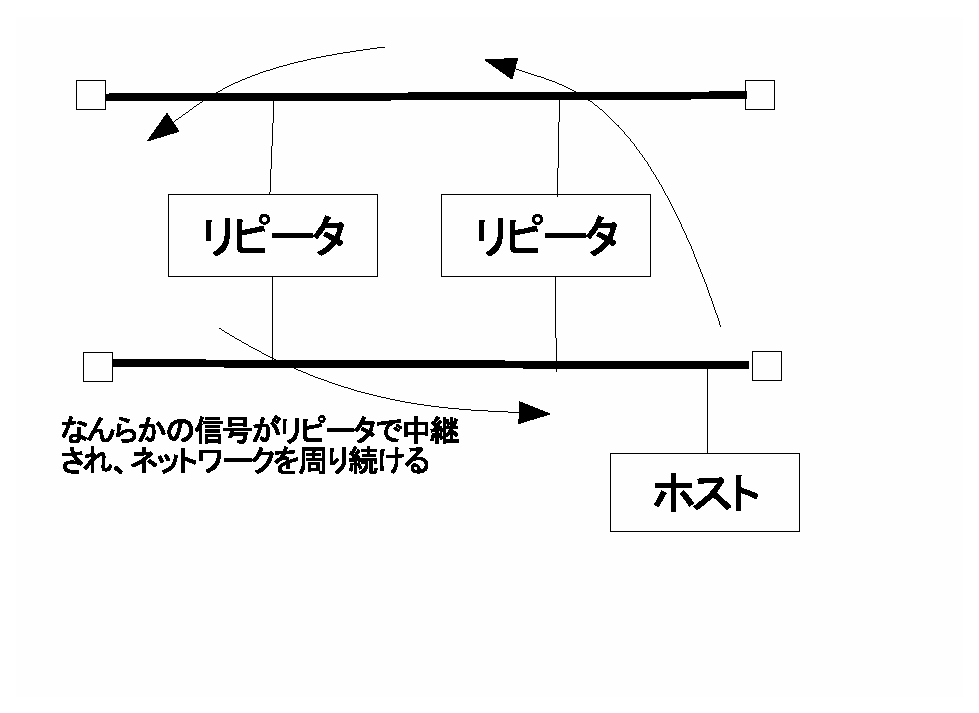
\includegraphics[width=10cm,clip]{draw/repeaterloop.eps}
	\caption{リピータによるループ}
	\label{fig:repeaterloop}
\end{figure}

最初に、イーサネットのループをリピータで作った場合について考えてみよう。たとえば、リピータの両端を同じ同軸ケーブルに接続したり、リピータHUBに接続したLANケーブルを、同じリピータHUBの別の口に接続したような場合である。

繰り返すが、リピータ(リピータHUB)で接続されたネットワークは、CSMA/CDで共有伝送媒体を管理するネットワークであり、同一の衝突ドメインである。

そのどこかでフレームが送信されたとしたら、リピータはそれを中継する。そうすると、ループの中でフレームが周りつつける現象がはっせいする。そうなると、その衝突ドメインに接続されているホストは全て、CSMA/CDに従い、信号がなくなるのを待ち続ける。

その結果、その衝突ドメイン内でのフレームの送信ができなくなる。これが、リピータでループを作ったときに発生する現象である。

\subsection{ブリッジによるループ}

では、ブリッジでループを作るとどうなるか。独立した衝突ドメインが二つ、ブリッジによってリング状に接続されている状況を想定してみよう。

ブリッジでループを作ると、イーサネットフレームが同じネットワークの中を回り続ける現象が発生する。この現象は、ブロードキャストストームと呼ばれる。では、ブロードキャストフレームはどのように生ずるのだろうか。

まず、二つの衝突ドメインを、二つのブリッジで並列に接続した場合を考える。この場合、二つのブリッジが、イーサネットでブロードキャストするフレームを転送し続ける「転送ループ」が生じる。

それぞれの衝突ドメインを、A、Bとして例を示そう。衝突ドメインAで送信されたフレームは、時間差はあっても二つのブリッジに到着する。2台のブリッジの学習が十分でない、もしくはブロードキャストアドレス宛の送信であったなどの理由で、フレームは衝突ドメインBに投げられる。

そのフレームは衝突ドメインB内でブロードキャストされているので、それぞれもう一方のブリッジで受信される。そのブリッジが、衝突ドメインA側のMACアドレスの学習が十分でない、フレームの宛先がブロードキャストアドレスであった、などの理由で、フレームが衝突ドメインAに向けて送信される。

ブリッジはMACアドレスが「どの衝突ドメインから来たか」学習するので、同一のフレームが回り続けると、二つの衝突ドメインの双方に、そのフレームの送信元MACアドレスのホストが存在する、という誤った学習がされてしまう。それによって、MACアドレスの学習テーブルが異常となり、最終的に、ブリッジを越える通信ができなくなる。この現象を、ブリッジのMACアドレスのテーブルが、誤った情報で汚染されることから、MACポイズニングという。

また、同一のフレームが再送信され続けるので、ループ内の通信トラフィックが徐々に増加していく。ブリッジは電気信号の正帰還による発振は発生しない。だが、中継処理の過負荷で故障する可能性がある。

\begin{figure}[htbp]
	\includegraphics[width=12cm,clip]{draw/bridgeloop.eps}
	\caption{誤学習とブロードキャストストームの発生}
	\label{fig:bridgeloop}
\end{figure}


\subsection{スイッチングHUBによるループ}

衝突ドメインがポート毎に独立しているスイッチングHUBでネットワークのループを作ると何が起こるのであろうか。たとえば、一本のLANケーブルの両端を、同じスイッチングHUBの別のポートに接続した場合を考えてみよう。。

この場合、そのスイッチングHUB2接続されたホストから、ブロードキャストフレームなどの、全てのポート宛に送信されるフレームが送信されたとき、問題が発生する。そのフレームがループ接続されているポートに向けて送信されたとき、ループを通って再度別のポートから同じフレームが「送信されてくる。

そうすると、このフレームを再度全ポートに向けて送信し直す転送ループが発生し、通信量が増加していく。もしこのスイッチングHUBが別のHUBに接続されているとすれば、そのHUBへも拡大再生産されるトラフィックをばらまくことになる。この現象を、ブロードキャストストームと呼んでいる。

また、ループによって、先だって説明したMACポイズニングが発生し、正しいポートへの転送ができなくなる、という問題も生じる。

\subsection{イーサネットのループと冗長化}
たった一カ所のループで同じネットワークの通信が実質的に不可能になるのが、イーサネットの最大の弱点である。

イーサネットでは、ネットワーク上にループを作ってはならない。繰り返すが、イーサネットがイーサネットであることに由来する、唯一最大の弱点である。またこれは、イーサネットは、そのままでは複数の経路による冗長化ができない、ということでもある。

逆に言えば、イーサネットにおいて、ループができたとき自動的にそれを回避することと、複数の経路による冗長化を実現することは、同じ意味を持つわけだ。

ループの回避と冗長化を実現する方法として、802.1Dスパニングツリーアルゴリズムという規格が存在する。本書では、スパニングツリーについては、詳細には立ち入らない。そんな方法があるとだけ覚えておいてもらい、普段はループを作らないことに気をつけてもらいたい。

\section{イーサネットの規格}

ここまでで紹介したものでも、イーサネットには、伝送媒体に同軸ケーブルを使用するもの、HUBとLANケーブルを使用するものがあった。実際、これまでの説明では、同軸ケーブルを使う、LANケーブルとHUBを使う、など、主に伝送媒体の種類でイーサネットの規格を区別してきた。

今度はそれを、イーサネットの規格名で表してみることにしよう。イーサーネットの規格は、Mbps単位の通信速度、フレームのビット列の変調方式、通信媒体の種類もしくはネットワークの1セグメント最大長\footnote{同軸ケーブルを使用する規格では、100を単位として表す。それ以外のケーブルを使う規格では、ケーブル長は規格名称に用いない。}というルールになっている。

歴史的経緯のあるものも含め、使用されることの多い規格をいくつか紹介する。ここでは省略したが、イーサネットには、光ファイバを伝送媒体として使用する規格もある。光ファイバの利点は、一般にセグメント距離が同じ速度の規格で使用する電気ケーブル\footnote{通信の分野では、金属線、銅線という意味で「メタル」「カッパー」という用語を用いる}よりも長くすることができる点である。たとえば、ビルのバックボーン\footnote{上下のフロアを貫く、縦方向の共用導管}を経由する接続など、 100メートル以上ケーブルを敷設しなければならない場合などに使用される。

\begin{table}[htbp]  \label{ethernet}
\begin{center}
\begin{tabularx}{110mm}{XXXXXX} \toprule
規格名 & 俗称 & 通信速度 & ケーブル & セグメント距離 & 全二重\\ \midrule
10Base2 & Thin Eternet & 10Mbps & 50Ωシン同軸ケーブル(5mm) & 185m & なし \\
10Base5 & Thick Ethernet & 10Mbps & 50Ωシック同軸ケーブル(12mm) & 500m & なし \\
10BaseT &- & 10Mbps & UTP/STP Cat.3,4,5 & 100m & あり\\
10Broad36 & - &10Mbps & 75Ω同軸ケーブル & 3600m & なし\\
100BaseTX & Fast Ethernet & 100Mbps & UTP Cat.5 & 100m & あり\\
1000BaseT &Gigabit Ether GbE & 1000Mbps & UTP Cat5e & 100m & あり\\
10GBaseT & - & 10Gbps & UTP Cat6 & 100m & 必須\\ \bottomrule
\end{tabularx}
\end{center} \caption{イーサネットの規格}
\end{table}

\begin{figure}[htbp]
	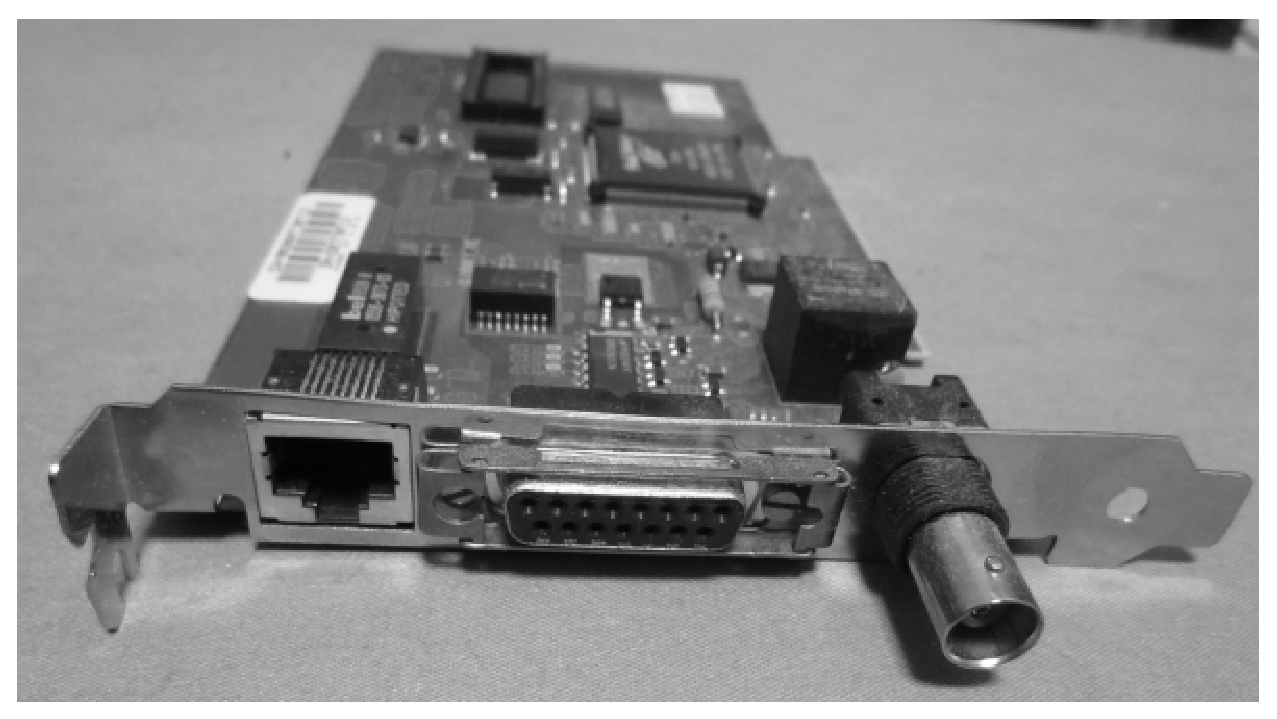
\includegraphics[width=12cm,clip]{draw/3com.eps}
	\caption{3Com EtherLink III PCI}
	\label{fig:3com}
\end{figure}

図\ref{fig:3com}は、左から10BaseT、10Base5(AUI)、10Base2の、三つのイーサネット規格のインタフェイスを搭載したネットワークカード、3ComのEtherLink III PCIである。

\subsection*{}
\begin{itembox}[l]{いもうとコラム 1000BaseTX}
ギガビットイーサネットの規格名は、1000BaseTです。1000BaseTは、4対のツイストペア全てを使って通信します。それぞれのツイストペアを、通信の上り下りで共用し、250Mbpsの速度で通信を行います。それによって、トータルで、全二重1Gbpsの速度を出しています。

ですが、4対のツイストペアのそれぞれを上り下りで共用する、ということは、ツイストペアごとの送受信回路と、送受信の信号を分離する回路とが必要になります。これはGbE製品が出始めた頃は、ネットワーク機器のコストを押し上げる一因と考えられていました。

そこで提案されたのがもう一つのGbE規格、1000BaseTXです。1000BaseTXは、ネットワーク機器を構成する部品を減ら氏、コストダウンすることを目的として、提案されました。

1000BaseTXは、4対のツイストペアを、2対づつ、上り専用、下り専用で使い分けます。そして、各ツイストペアで500Mbpsの速度で通信を行い、全体で全二重1Gbpsの速度を出します。
そして、ツイストペアごとに500Mbpsの通信を可能とするLANケーブルとして、イソレータ入りケーブルのCat.6の規格が定められました。

理屈の上では1000BaseTXは、Cat.6を必要とするケーブルのコストは高いものの、部品点数の少なくなるネットワーク機器のコストは安い、という規格になるはずでした。ですが、1000BaseT対応機器の価格が予想よりも速いペースで下がったことから、1000BaseTXは対抗機器が市販されることなく消えていきました。

いまでは、1000BaseTXは、Cat.6ケーブルにその名残を残すだけです。Cat.6ケーブルは、1000BaseTでも使用できるもの、電気信号レベルでは非互換で、相互接続性がありません。そのため、機器が販売されていたら、1000BaseTと相互接続できないことに起因する問題を起こしていたでしょう。


\end{itembox}


\section{ベースバンドとブロードバンド}

イーサネット規格の名称には、BASEとBROADの二種類があった、これは何を表すものでであろうか。

まず、規格上は10BROAD36に名を残すのみであるBROADについて説明しよう。BROADは、広帯域変調(ブロードバンド変調)であり、WANの速度が速いという意味で誤用されているブロードバンドとではない。では、変調とはなにか。変調とは、伝送したい信号よりも、伝送媒体での伝播特性がよい周波数の信号に、伝送したい信号をのせて送り出すことである。この、伝送特性が良い周波数の信号を、搬送波(キャリア)という。

ラジオのAMやFMというのも、それぞれ、振幅変調(Amplifire Modulation)、周波数変調(Frequency Moduulation)、という変調方式の名称からきている。

一方のBASEとはベースバンド方式という伝送方法になる。ベースバンド方式は、伝送したい信号を変調せずにそのまま伝送媒体に流す。例えば、アナログ電話は変調を行わないのでベースバンド伝送である。また、ステレオミニプラグからヘッドフォンまでのオーディオケーブルに流れる信号も、出力する音声そのものなので、ベースバンドで伝送している信号である。

イーサネットの規格のほとんどは、フレームのビット列から伝相場いたで送信しやすい波形を作った上で、それを変調せずにそのまま電気信号として流す、ベースバンド方式を用いている。

イーサネットでブロードバンド変調を行うのは、CATV向けの同軸ケーブルに、テレビ電波と一緒に信号を送信する規格である10BROAD36のみである。\footnote{余談ながら、フレッツTVという形で、インターネット接続、電話線、ケーブルテレビの重畳を行う通信が復活していることは興味深い}

\subsection{ベースバンドと符号化}

ベースバンド方式を用いるイーサネットの規格では、ビット列の1と0でそのまま信号をオンオフしているのではないかと、ここまでの説明で考えたかもしれない。ベースバンド方式では、ビット列を何らかの形で時系列方向の電圧の変化に置き換える必要がある。この置き換えを、符号化と呼んでいる。

一番簡単な方法として、先に挙げたように、1のときだけ信号を流して0の時は信号を流さない、というやり方が考えられる。だが、この方法は実用的ではない。なぜなら、送受信の双方で、何らかの方法で、タイミングの同期を図る必要がある。そうでなければ、1や0が連続したとき、いくつ1や0が続いていたのかが分からない。だが、イーサネットでは、複数のノードが同期した時計を共有する、という仕組みは持っていない。

次に、1を電圧のH、0を電圧のLとする2値符号方式が考えられるだろう。だが、これも、送受信する双方でクロックの同期が必要となる。なぜなら、これも同じ値が続けば、同じ値のビットが連続したときに、いくつそれが続いていたのかわからなくなる。

では、実際にはどのような符号化の方法が採られているのであろうか。ここでは10BaseTで使用されるマンチェスター符号と100BaseTXで使用される4B5B+MLT-3についてごく簡単に説明しよう。

\subsubsection{マンチェスター符号化}
マンチェスター符号は、電圧がHからLに変化する場合は0、LからHに変化する場合を1として扱う符号化方式である。1でも0でも、1ビットの信号のうちにかならず電圧の変化が生じる。送信側と受信側での信号の同期には、その電圧変化をクロックとして用いることができる。

マンチェスター符号化の欠点は、信号の電圧変化が大きいことである。では、これがなぜ欠点になるのであろうか。マンチェスター符号をフーリエ変換して周波数成分をもとめると、それを構成する周波数の成分が多い。つまり、周波数の幅が広い。\footnote{この周波数の幅を、側波帯という。}。これは、影響を受けるノイズの周波数が多いということであり、ノイズに弱いということである。そのため、マンチェスター符号は、100Mbpsのイーサネットでは使用することができない。

\begin{figure}[htbp]
	\includegraphics[width=12cm,clip]{draw/manchester.eps}
	\caption{マンチェスター符号と4B5B+MLT3}
	\label{fig:manchester}
\end{figure}

\subsubsection{4B5B+MLT5}
では、100BaseTXで使用される4B5B+MLT-3という符号化はどういうものか説明しよう。マンチェスター符号が、構成する周波数成分が多くて100Mbpsで使用できないということであったので、周波数成分が狭いのではないかという予想がつく。たしかに、4B5B+MLT-3は、マンチェスター符号化より周波数成分が狭い。

4B5B+MLT-3とは、連続する4ビットを5ビットに変換する、4B5Bマッピングと、MLT-3という符号化方式を組み合わせた符号化方式である。

MLT-3とは、三値の状態を持つ。そして、1で電圧が上下に一つ変化、0は変化なしという符号化である。この方式は電圧変化がマンチェスター符号よりゆるやかであるため、フーリエ変換した際に、構成する周波数が少ない。つまり、影響を受けるノイズの周波数が少ないということであり、比較的ノイズに強い。

だが、この符号化方式では、0が連続すると同期がとれなくなる。そのため、4ビットを5ビットにマッピングし、連続する5ビットのうち1が二つ以上入るようにする。これが、4B5Bという名称の理由である。\footnote{4B5Bは、変換表で変換する。変換表については本書では割愛するが、必要であれば電気通信の教科書などを参照して欲しい。}

100BaseTXでは、この二つの符号化方式を併用する。そのため、符号化方式の名称が4B5B+MLT-3となる。

\subsubsection{ギガビットイーサネットの符号化方式}
ギガビットイーサネットでは、8B1Q4+4D-PAMという符号化方式を用いる。8B1Qは、8ビットをエラー訂正ビットを加えた9ビットにマッピングし、5進数(Quinary)4桁であらわす。

8B1Qは、エラー訂正ビットを含めた9bitの先頭3bitから、残り6bitの変換表を決定し、5進数4桁に変換する。実際に、9bitは0から511まで、5進数4桁は0から624まで表現することができるので、9bitをマッピングすることが可能である。

4D-PAM5では、その4桁の5進数の核桁を、LANケーブルの4組あるツイストペアに対応させる。それによって、全てのツイストペアを使って、8bitを一度に送出する。

\subsection*{}
\begin{itembox}[l]{いもうとコラム 無線通信のベースバンド方式}
ここまで、イーサネットで用いる、有線通信でのベースバンド方式について見てきました。では、、無線通信におけるベースバンド方式とはどのようなものなのでしょうか。

無線で、ベースバンド方式の送信機は、マルコーニが実用化した火花送信機と、その改良型しか存在しません。火花送信機とは、スイッチのオンオフによる電流のオンオフを、そのままコイルで誘導電流のオンオフとします。そのコイルは放電電極に接続されています。そして、放電電極からの火花放電による電磁波をアンテナから放出するという仕組みです。

火花送信機から発射される電波はホワイトノイズです。つまり帯域幅がものすごく広いため、現在のように細かく周波数を区切ってその用途を指定する電波の使い方をする際の障害となってしまいます。なので、、1955年以降は、国際電気通信条約付属無線規則で使用が禁止されました。

日本に現存する火花送信機は、三六式無線機です。これは戦艦三笠に搭載されていました。実物は東京都墨田区の郵政博物館に収蔵されています。また、横須賀の記念艦三笠では、三六式無線機のレプリカが展示されています。

最後に余談ながら、誤解されていることも多いですが、現代の、モールス信号による無線通信のための送信機は、搬送波にキーのオンオフを印加した変調波で通信を行っています。
\end{itembox}


\section{イーサネットフレーム}

ここまで、ネットワークアクセス層にイーサネットを使用した場合の送出単位、という意味で、イーサネットフレームという用語を使用してきた。では、イーサネットフレームの構造について説明しよう。。

イーサネットフレームは、イーサネットに送出されるデータの単位である。イーサネットフレームの長さは、64オクテットから1518オクテットまでの可変長となる。ここで、オクテット(octet)という表現を用いたが、意味はbyteとおなじ、8bitを単位としたデータ量である。\footnote{デー通信では、9ビットの単位として、byteでなく、octetを用いることがある。ネットワークアクセス層以下では、オクテットと呼ばれることが多い。}

イーサネットフレームの構造は、図\ref{fig:etherframe}のように表すことができる。。

\begin{figure}[htbp]
	\includegraphics[width=14cm,clip]{draw/ethernetframe.eps}
	\caption{イーサネットフレーム}
	\label{fig:etherframe}
\end{figure}


\begin{description}
\item[プリアンプル]信号を共有チャネルを使用するデバイスが認識する時間をとるためのリード。最近のコンスタントシグナリングを使用する規格では実質的に使用しないが、フレーム構造の維持のためにつけられる
\item[宛先アドレス]データの宛先ネットワークインタフェイスのMACアドレス
\item[発信元アドレス]データの発信元ネットワークインタフェイスのMACアドレス
\item[タイプ/長さ]1500より小さい数のときはデータのオクテット長。1536より大きい数のときは上位プロトコルの種類を表すフィールドとなる。
\item[データ]46octet~1500octetの可変長。イーサネットフレームに乗せるデータを1500octet以内の大きさにするのは上位プロトコルの役目
\item[フレームチェックシーケンス(FCS)]CRCによって、プリアンプルを除くフィールドの値にエラーが生じていないかをチェックする。文献によっては、FCSではなくCRCと記載していることがある。
\end{description}

イーサネットフレームの最小の大きさは64オクテット(512bit)となる。これは、10Base5における線路長の最大が2500メートル\footnote{500メートルの同軸ケーブルからなるセグメント3本を、500メートル長の渡り線をもつリピータ2台で接続してひとつの衝突ドメインとした場合の数字である。}であることから決定された。


受信した情報にエラーが生じている可能性があっても、Ethernetのには再送やそのリクエスト機能はない。単に、該当するフレームを破棄するのみである。あるフレームが破棄された場合に、再送するかどうかを判断するのは、ネットワークアクセス層よりも上位プロトコルの役目である。

\subsection{MTUとフラグメント}

先ほど、イーサネットフレームの最小の大きさが64オクテットであるという説明を行った。では、逆に、フレームの最大の大きさというのはどのように決定されるのであろうか. 

二章に分けて行ったネットワークアクセス層に関する話題の最後に、フレームの大きさを決定するMTUと、MTUに起因するフラグメントについて簡単に説明を行なおう。

ネットワークアクセス層のフレームにおける、データ部分の最大の大きさを、MTU(Maximum Transmission Unit 最大転送単位)という。MTUは、イーサネットに限らず、全てのネットワークアクセス層に存在する概念である。たとえば、イーサネットやPPPのMTUは 1500でとなる。

例外がSLIPで、これはIPデータグラムをそのまま流すものであるため、ネットワークアクセス層としてのMTUの概念がない。\footnote{後ほど改めて説明するが、IPv4の場合、IPデータグラムの最大のサイズである64Kbyteが、その最大サイズであると言うこともできる。}

MTUとは、そのネットワークアクセス層で、一度の送信によって運ぶことができるデータ量の上限である。つまり、送信するデータが、通信に使用するネットワークアクセス層のMTUより大きい場合には、データのサイズをMTUよりも小さくなるように分割し、受信側ではその切片を集めて元のデータを取り出さなければならない。これがフラグメントである。

\subsubsection{フラグメント}
ネットワークアクセス層には、データを分割(フラグメント)したり、フラグメントされたデータを元に戻したりする機能がない。データを元に戻せるように分割(フラグメント)し、フラグメントを集めて元に戻すことを担当するのは、上位層である。

フラグメントを担当する層は、IPv4とIPv6で異なる。
IPv4でフラグメントを担当するのは、インターネットプロトコル層である。トランスポート層にはパスMTUディスカバリという機能があり、経路のMTUを検出することが可能である。そして、基本機能としてフラグメントが実装されているのはインターネットプロトコル層となる。

\subsubsection{最小MTU}
上位層にIPv6を使用する場合、最小MTUというものが規定されている。最小の「最大転送単位」というのも変なものだが、上位プロトコルの都合で、MTUとして最低限確保しなければならないデータサイズのことである。

上位にIPv6を使用する場合は、1280byteが最小となる。IPv4には明確な規定はないが、あえていうならヘッダ長20byteにデータ長をくわえた長さになる。

\subsection{タイプ・長さフィールド}
イーサネットフレームの中には、タイプ・長さというフィールドがある。十進数で1500以下ならオクテット長としてのサイズ、1536以上ならデータ部分がどのプロトコルのデータであるかを洗わすタイプとなる。
この違いは、かつてDIX\footnote{DEC,Intel,Xerox}仕様とも呼ばれた初期のイーサネットと、DIX仕様を基としてIEEEで規格化された802.3との相違によって生じたものである。

DIX仕様では、このフィールドは、フレームがどの上位プロトコルのデータをカプセル化しているかを表すものである。たとえば、IPv4IPアドレスを持つデータグラムであれば、十六進数で0800(十進数で2048)を入れる。これで判るように、DIX仕様の時は、イーサネットのフレームにはデータ長を表すフィールドがなかった。

一方、IEEE802.3では、このフィールドはデータ部分のオクテット長でのサイズとなる。では、逆にデータのタイプフィールドはどこに行ったのだろうか。802.3規格では、データ部分の先頭に、タイプなどの付加情報を付加するというものであった。

DIX仕様のフレームと802.3のフレームは、このフィールドを見ることで区別することができる。実際の機器は、この二つの形式のフレームをどちらも同様に取り扱うことが可能である。

もっとも、現在は、上位層はインターネットプロトコルでほぼ決め打ちすることができる。そのため、このフィールドは長さとして使う802.3方式だが、データのタイプを表すヘッダを省略したDIX仕様方式、という折衷的なフレームが用いられることが多い。\footnote{実のところ、これは過去にNovel 802.3Rawと呼ばれた規格と同じ形式である。Novellが802.3ドラフトを基に、イーサネットでIPXのデータを伝送するために定めた規格が後に、このように呼ばれた。上位層のプロトコルをIPXで決め打ちとしたため、データタイプのフィールドが省略された。}



\subsection{ジャンボフレーム}
ギガビットイーサネットでは、接続可能なネットワークの総延長をかせぐために、フレームのサイズを大きくする。つまり、送出する時間を延ばすという方法をとる。

それであれば、イーサネットフレームのペイロードそのものを大きくしてしまっても、同じである。その考えで、ペイロードを大きくしたイーサネットフレームを、ジャンボフレームと呼ぶ。

ジャンボフレームはイーサネットの規格で正式に定められたものではなく、ベンダ規格である。そのため、接続する危機感では、互換性がとれず、ジャンボフレームで通信できないことがある。


\subsection*{}
\begin{itembox}[l]{いもうとコラム PPPoE}
先に説明したPPPは、接続手順、認証機能、切断手順が存在します。これらの機能は、伝送媒体がなにであるかにかかわらず、必要となる場合があります。

接続時認証や、接続・切断をイーサネットの上で制御したいときは、イーサネットの上でPPPを用いることで実現できます。この、イーサネットの上でPPPによる接続を行うこのが、RFC2516で提案されたPPPoE(PPP on Ethernet)です。\footnote{ただし、PPPoEのPPPヘッダは、シリアル(電話線)で使用するPPPとは異なります。PPPoEは、PPPのフレームをそのままイーサネットに乗せているわけではありません。 }

たとえば、NTT東西のインターネット接続サービスであるフレッツADSLやB-Fletsは、プロバイダとの接続のためのプロトコルとして、PPPoEが用いられています。

PPPoEでは、イーサネットフレームの上に、PPPのフレームを押し込んで通信します。当然ながら、PPPoEを用いた場合、PPPoEのフレームの中にインターネットプロトコル層から渡されたフレームを詰め込むので、それによるオーバヘッドが生じます。

\end{itembox}


